\documentclass[a4paper,10pt]{article}
\usepackage[utf8]{inputenc}
\usepackage[english]{babel}
\usepackage{fontenc}
\usepackage{graphicx}
\usepackage{amsfonts}
\usepackage{hyperref}
\usepackage{amssymb}
\usepackage{fullpage}
\usepackage[ruled,vlined,linesnumbered]{algorithm2e}
\usepackage{float}
\usepackage{amsthm}
\usepackage{amsmath}
\usepackage{amssymb}
\usepackage{mathrsfs}
\providecommand{\SetAlgoLined}{\SetLine}
\providecommand{\DontPrintSemicolon}{\dontprintsemicolon}
\title{Using Bloom Filters to merge Dags}
\author{Matthieu JOURNAULT}
\date{24/06/2013}
\theoremstyle{definition}
\newtheorem{lemma}{Lemma}
\newtheorem{proposition}{Proposition}
\newtheorem{definition}{Definition}
\theoremstyle{definition}
\usepackage{tikz}
\usetikzlibrary{arrows}
\usepackage{fullpage}
\definecolor{turquoise}{RGB}{255,127,0}
\tikzset{
  treenode/.style = {align=center, inner sep=0pt, text centered,
    font=\sffamily},
  arn_ns/.style = {treenode, rectangle, white, font=\sffamily\bfseries, draw=black,
    fill=black, minimum width=1.5em, minimum height=1.5em, very thick},% arbre rouge noir, noeud noir
  arn_n/.style = {treenode, circle , white, font=\sffamily\bfseries, draw=black,
    fill=black, text width=1.5em},% arbre rouge noir, noeud noir
  arn_r/.style = {treenode, circle , red, draw=red, 
    text width=1.5em, very thick},% arbre rouge noir, noeud rouge
  arn_x/.style = {treenode, rectangle, draw=black,
    minimum width=1em, minimum height=1em},% arbre rouge noir, nil
  arn_b/.style = {treenode, circle , blue, draw=blue, 
    text width=1.5em, very thick},
  arn_g/.style = {treenode, circle , green, draw=green, 
    text width=1.5em, very thick},
  arn_y/.style = {treenode, circle , yellow, draw=yellow, 
    text width=1.5em, very thick},
    arn_pu/.style = {treenode, circle , purple, draw=purple, 
    text width=1.5em, very thick},
    arn_pi/.style = {treenode, circle , pink, draw=pink, 
    text width=1.5em, very thick},
    arn_t/.style = {treenode, circle , pink, draw=turquoise, 
    text width=1.5em, very thick},
    arn_rb/.style = {treenode, circle , red, draw=red, 
    text width=2.5em, very thick},
    arn_bs/.style = {treenode, rectangle , blue, draw=blue, 
    minimum width=1.5em, minimum height=1.5em, very thick},
    arn_rs/.style = {treenode, rectangle, red, draw=red, 
    minimum width=1.5em, minimum height=1.5em, very thick},% arbre rouge noir, noeud rouge
  arn_gs/.style = {treenode, rectangle , green, draw=green, 
    minimum width=1.5em, minimum height=1.5em, very thick},
  arn_ys/.style = {treenode, rectangle , yellow, draw=yellow, 
    minimum width=1.5em, minimum height=1.5em, very thick},
    arn_pus/.style = {treenode, rectangle , purple, draw=purple, 
    minimum width=1.5em, minimum height=1.5em, very thick},
    arn_pis/.style = {treenode, rectangle , pink, draw=pink, 
    minimum width=1.5em, minimum height=1.5em, very thick},
    arn_rbs/.style = {treenode, rectangle , red, draw=red, 
    minimum width=1.5em, minimum height=1.5em, very thick},
    arn_ts/.style = {treenode, rectangle, pink, draw=turquoise, 
    minimum width=1.5em, minimum height=1.5em, very thick},
    }% arbre rouge noir, noeud rouge}
\begin{document}
\maketitle
\section{Algorithm}
\begin{algorithm}[H]
  \SetAlgoLined
  \caption{Finding some of the ancestors of $Alice$ not known by $Bob$}
  \SetKwInOut{Input}{input}\SetKwInOut{Output}{output}
  \SetKwComment{tcc}{(*}{*)}
  \KwData{\texttt{Alice\_Heads} : some nodes in the history of $Alice$, \texttt{Ancestor} : a dag of the ancesters of $Alice$, \texttt{G\_In} : a graph of ancestors of $Alice$ not known by $Bob$, \texttt{Bf} : The Bloom filter of $Bob$, \texttt{Bd} : The Border of $Bob$}
%   \KwData{
%     \begin{itemize}
%     \item \texttt{Alice\_Heads} : some nodes in the history of $Alice$
%     \item \texttt{Ancestor} : a dag of the ancesters of $Alice$
%     \item \texttt{G\_In} : a graph of ancestors of $Alice$ not known by $Bob$
%     \item \texttt{Bf} : The Bloom filter of $Bob$
%     \item \texttt{Bd} : The Border of $Bob$
%     \end{itemize}
%     }
  \KwResult{\texttt{G\_Out} : a graph of ancestors of $Alice$ not known by $Bob$, \texttt{node\_to\_check} : a list of ancestors of $Alice$ that shall be revisited with the next Bloomfilters}
%   \KwResult{
%   \begin{itemize}
%   \item \texttt{G\_Out} : a graph of ancestors of $Alice$ not known by $Bob$
%   \item \texttt{node\_to\_check} : a list of ancestors of $Alice$ that shall be revisited with the next Bloomfilters
%   \end{itemize}
%   }
  
\SetAlgoLined\DontPrintSemicolon
\SetKwFunction{explore}{\textbf{explore}}
\SetKwFunction{belong}{\textbf{belong}}
\SetKwFunction{addv}{\textbf{add\_vertex}}
\SetKwFunction{adde}{\textbf{add\_edge}}
\SetKwFunction{succ}{\textbf{successor}}
\SetKwFunction{pred}{\textbf{predecessor}}
\SetKwProg{myproc}{Procedure}{}{}
\myproc{\explore{\texttt{node},\texttt{visited},\texttt{in\_bf},\texttt{in\_border}}}{

  \eIf{\belong{\texttt{node,\texttt{Bf}}}}{
    \KwRet{(\texttt{visited} $\cup$ \texttt{node},\texttt{in\_bf} $\cup$ \texttt{node},\texttt{in\_border})}
  }
  {
    \eIf{\belong{\texttt{node,\texttt{Bd}}}}{
    \KwRet{(\texttt{visited} $\cup$ \texttt{node},\texttt{in\_bf} ,\texttt{in\_border}$\cup$ \texttt{node})}
    }
    {
      \texttt{visited\_already} = \texttt{node} $\cup$ \texttt{visited}\;
      \texttt{in\_bf\_already} = \texttt{in\_bf}\;
      \texttt{in\_border\_already} = \texttt{in\_border}\;
      \For{\texttt{pere} $\in$ \pred{\texttt{Ancestor},\texttt{node}}}{
      \If{\texttt{pere} $\notin$ \texttt{explored}}
      {
	\texttt{visited\_already,in\_bf\_already,in\_border\_already} = \explore{\texttt{pere},\texttt{visited\_already},\texttt{in\_bf\_already},\texttt{in\_border\_already}}\;
      }
      }
      \KwRet{(\texttt{visited\_already},\texttt{in\_bf\_already},\texttt{in\_border\_already})}\;
    }
  }
}

\SetKwFunction{bf}{\textbf{find\_in\_bf}}
\SetKwFunction{bd}{\textbf{find\_in\_border}}
\myproc{\bf{\texttt{node},\texttt{explored}}}{
    \addv{\texttt{G\_In},\texttt{node}}\;
    \texttt{already\_explored} = \texttt{explored} $\cup$ \texttt{node}\;
    \For{\texttt{fils} $\in$ \succ{\texttt{Ancestor},\texttt{node}}}{
      \adde{\texttt{G\_In},\texttt{node},\texttt{fils}}\;
      \If{$\texttt{fils} \notin \texttt{already\_explored} \wedge \texttt{fils} \notin \texttt{G\_In}$}{
	\texttt{already\_explored} = \bf{\texttt{fils},\texttt{already\_explored}}
	}
    }
    \KwRet{already\_explored}
}

\myproc{\bd{\texttt{node},\texttt{explored},\texttt{to\_further\_explore}}}{
  \If{$\texttt{node} \notin \texttt{explored}$}{
    \texttt{son\_in} = $\varnothing$\;
    \texttt{son\_out} = $\varnothing$\;
    \For{\texttt{fils} $\in$ \succ{\texttt{Ancestor},\texttt{node}}}{
      \eIf{\texttt{fils} $\in$ \texttt{G\_In}}{
	\texttt{son\_in} = \texttt{fils} $\cup$ \texttt{son\_in}\; 
      }{
	\texttt{son\_out} = \texttt{fils} $\cup$ \texttt{son\_out}\;
      }
    }
    \texttt{already\_explored} = \texttt{explored}\;
    \texttt{inter\_node} = \texttt{to\_further\_explore}\;
    \If{\texttt{son\_in} = $\varnothing$}{
      \texttt{inter\_node} = \texttt{node} $\cup$ \texttt{inter\_node}\;
    }
    \For{\texttt{fils} $\in$ \texttt{son\_out}}{
      \If{\texttt{fils} $\notin$ \texttt{already\_explored}}{
	\texttt{already\_explored},\texttt{inter\_node} = \bd{\texttt{fils},\texttt{already\_explored},\texttt{inter\_node}}\;
      }
    }
    \KwRet{(already\_explored,inter\_node)}\;
  }
}
\end{algorithm}
  \begin{algorithm}
  \SetAlgoLined
  \caption{Finding some of the ancestors of $Alice$ not known by $Bob$}
  \SetKwInOut{Input}{input}\SetKwInOut{Output}{output}
  \SetKwComment{tcc}{(*}{*)}
  \KwData{\texttt{Alice\_Heads} : some nodes in the history of $Alice$, \texttt{Ancestor} : a dag of the ancesters of $Alice$, \texttt{G\_In} : a graph of ancestors of $Alice$ not known by $Bob$, \texttt{Bf} : The Bloom filter of $Bob$, \texttt{Bd} : The Border of $Bob$}
%   \KwData{
%     \begin{itemize}
%     \item \texttt{Alice\_Heads} : some nodes in the history of $Alice$
%     \item \texttt{Ancestor} : a dag of the ancesters of $Alice$
%     \item \texttt{G\_In} : a graph of ancestors of $Alice$ not known by $Bob$
%     \item \texttt{Bf} : The Bloom filter of $Bob$
%     \item \texttt{Bd} : The Border of $Bob$
%     \end{itemize}
%     }
  \KwResult{\texttt{G\_Out} : a graph of ancestors of $Alice$ not known by $Bob$, \texttt{node\_to\_check} : a list of ancestors of $Alice$ that shall be revisited with the next Bloomfilters}
%   \KwResult{
%   \begin{itemize}
%   \item \texttt{G\_Out} : a graph of ancestors of $Alice$ not known by $Bob$
%   \item \texttt{node\_to\_check} : a list of ancestors of $Alice$ that shall be revisited with the next Bloomfilters
%   \end{itemize}
%   }
  
\SetAlgoLined\DontPrintSemicolon

  \texttt{explored} = $\varnothing$\;
  \texttt{in\_bf} = $\varnothing$\;
  \texttt{in\_border} = $\varnothing$\;
  \texttt{to\_further\_explore} = $\varnothing$\;
\SetKwFunction{explore}{\textbf{explore}}
\SetKwFunction{belong}{\textbf{belong}}
\SetKwFunction{addv}{\textbf{add\_vertex}}
\SetKwFunction{adde}{\textbf{add\_edge}}
\SetKwFunction{succ}{\textbf{successor}}
\SetKwFunction{pred}{\textbf{predecessor}}
\SetKwProg{myproc}{Procedure}{}{}
\myproc{\explore{\texttt{node}}}{

\If{\texttt{node} $\notin$ \texttt{explored}}
{
\texttt{explored} = \texttt{node} $\cup$ \texttt{explored}\;
\eIf{\belong{\texttt{node,\texttt{Bf}}}}{
  \texttt{in\_bf} = \texttt{node} $\cup$ \texttt{in\_bf}\;
  }
  {
  \eIf{\belong{\texttt{node,\texttt{Bd}}}}{
  \texttt{in\_border} = \texttt{node} $\cup$ \texttt{in\_border}\;
  }
  {
  \For{\texttt{pere} $\in$ \pred{\texttt{Ancestor},\texttt{node}}}{
    \explore{\texttt{pere}}
  }
  }
  }
}
}
\SetKwFunction{bf}{\textbf{find\_in\_bf}}
\SetKwFunction{bd}{\textbf{find\_in\_border}}
\myproc{\bf{\texttt{node}}}{
  \If{$\texttt{node} \notin \texttt{explored} \wedge \texttt{node} \notin \texttt{G\_In}$}{
    \addv{\texttt{G\_In},\texttt{node}}\;
    \For{\texttt{fils} $\in$ \succ{\texttt{Ancestor},\texttt{node}}}{
      \adde{\texttt{G\_In},\texttt{node},\texttt{fils}}\;
      \bf{\texttt{fils}}
    }
  }
}
\myproc{\bd{\texttt{node}}}{
  \If{$\texttt{node} \notin \texttt{explored}$}{
    \eIf{$\texttt{node} \in \texttt{G\_In}$}{
      \texttt{to\_further\_explore} = \texttt{node} $\cup$ \texttt{to\_further\_explore}\;
    }
    {
      \For{\texttt{fils} $\in$ \succ{\texttt{Ancestor},\texttt{node}}}{
      \bd{\texttt{fils}}
      }    
    }
  }
}
\For{\texttt{node} $\in$ \texttt{Alice\_Heads}}{
  \explore{\texttt{node}}
}
\texttt{explored} = $\varnothing$\;
\For{\texttt{node} $\in$ \texttt{in\_bf}}{
  \bf{\texttt{node}}
}
\texttt{explored} = $\varnothing$\;
\For{\texttt{node} $\in$ \texttt{in\_border}}{
  \bd{\texttt{node}}
}
\KwRet{(\texttt{G\_In,to\_further\_explore})}
  
  \end{algorithm}
\begin{figure}[H]
  \begin{minipage}{0.3\textwidth}
  \centering
  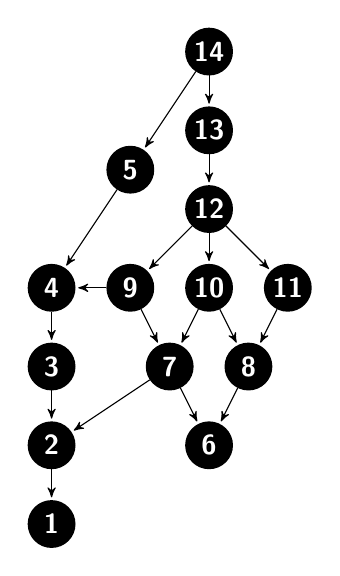
\begin{tikzpicture}[->,>=stealth',shorten >=1pt,auto,node distance=3cm,
  thick,main node/.style={circle,fill=blue!20,draw,font=\sffamily\Large\bfseries}]
  
  \foreach \place/\x in {{(0,0)/1}, {(0,1)/2},{(0,2)/3},{(0,3)/4}, {(1,4.5)/5}, {(2,1)/6}, {(1.5,2)/7},{(2.5,2)/8},{(1,3)/9},{(2,3)/10},{(3,3)/11},{(2,4)/12},{(2,5)/13},{(2,6)/14}}
  \node[arn_n] (a\x) at \place {\x};
%   Alice history
  \path[thin] (a14) edge (a5);
  \path[thin] (a5) edge (a4);
  \path[thin] (a4) edge (a3);
  \path[thin] (a3) edge (a2);
  \path[thin] (a2) edge (a1);
  \path[thin] (a9) edge (a4);
  \path[thin] (a7) edge (a2);
%   both history
  \path[thin] (a14) edge (a13);
  \path[thin] (a13) edge (a12);
  \path[thin] (a12) edge (a9);
  \path[thin] (a12) edge (a10);
  
  \path[thin] (a9) edge (a7);
  \path[thin] (a10) edge (a7);
%   Bob history
  \path[thin] (a12) edge (a11);
  \path[thin] (a11) edge (a8);
  \path[thin] (a10) edge (a8);
  \path[thin] (a7) edge (a6);
  \path[thin] (a8) edge (a6);
  \end{tikzpicture}
  \caption{Main Graph}
  \end{minipage}%
  \begin{minipage}{0.3\textwidth}
  \centering
  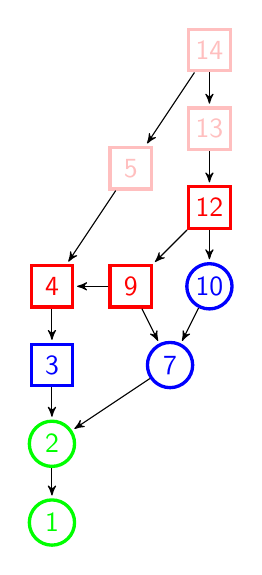
\begin{tikzpicture}[->,>=stealth',shorten >=1pt,auto,node distance=3cm,
  thick,main node/.style={circle,fill=blue!20,draw,font=\sffamily\Large\bfseries}]
  \foreach \place/\x in {{(0,0)/1}, {(0,1)/2}}
  \node[arn_g] (a\x) at \place {\x};
  
  
  \node[arn_pis] (a5) at (1,4.5) {5};
  \node[arn_pis] (a13) at (2,5) {13};
  \node[arn_pis] (a14) at (2,6) {14};
  
  
  \node[arn_b] (a10) at (2,3) {10};
  \node[arn_b] (a7) at (1.5,2) {7};
  \node[arn_bs] (a3) at (0,2) {3};
  
  \node[arn_rs] (a9) at (1,3) {9};
  \node[arn_rs] (a12) at (2,4) {12};
  \node[arn_rs] (a4) at (0,3) {4};
  %   Alice history
  \path[thin] (a14) edge (a5);
  \path[thin] (a5) edge (a4);
  \path[thin] (a4) edge (a3);
  \path[thin] (a3) edge (a2);
  \path[thin] (a2) edge (a1);
  \path[thin] (a9) edge (a4);
  \path[thin] (a7) edge (a2);
%   both history
  \path[thin] (a14) edge (a13);
  \path[thin] (a13) edge (a12);
  \path[thin] (a12) edge (a9);
  \path[thin] (a12) edge (a10);
  
  \path[thin] (a9) edge (a7);
  \path[thin] (a10) edge (a7);
  \end{tikzpicture}
  \caption{Alice's ancestors}
\end{minipage}%
\begin{minipage}{0.3\textwidth}
\centering
  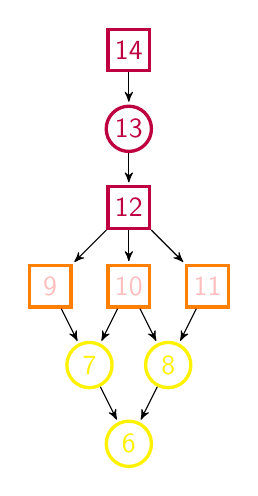
\begin{tikzpicture}[->,>=stealth',shorten >=1pt,auto,node distance=3cm,
  thick,main node/.style={circle,fill=blue!20,draw,font=\sffamily\Large\bfseries}]
%   
  \node[arn_y] (a6) at (2,1) {6};
  \node[arn_y] (a7) at (1.5,2) {7};
  \node[arn_y] (a8) at (2.5,2) {8};
  \node[arn_ts] (a9) at (1,3) {9};
  \node[arn_ts] (a10) at (2,3) {10};
  \node[arn_ts] (a11) at (3,3) {11};
  \node[arn_pus] (a12) at (2,4) {12};
  \node[arn_pu] (a13) at (2,5) {13};
  \node[arn_pus] (a14) at (2,6) {14};
  
%   both history
  \path[thin] (a14) edge (a13);
  \path[thin] (a13) edge (a12);
  \path[thin] (a12) edge (a9);
  \path[thin] (a12) edge (a10);
  
  \path[thin] (a9) edge (a7);
  \path[thin] (a10) edge (a7);
%   Bob history
  \path[thin] (a12) edge (a11);
  \path[thin] (a11) edge (a8);
  \path[thin] (a10) edge (a8);
  \path[thin] (a7) edge (a6);
  \path[thin] (a8) edge (a6);
  \end{tikzpicture}
  \caption{Bob's ancestors}

\end{minipage}
\end{figure}

\begin{figure}[H]
\begin{minipage}{0.3\textwidth}
\centering
 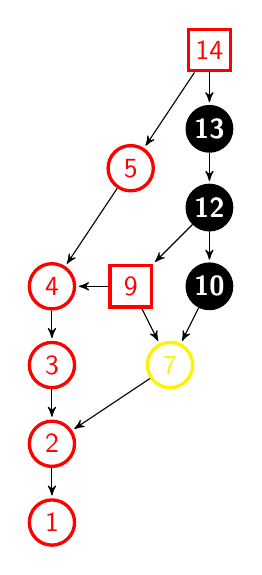
\begin{tikzpicture}[->,>=stealth',shorten >=1pt,auto,node distance=3cm,
  thick,main node/.style={circle,fill=blue!20,draw,font=\sffamily\Large\bfseries}]
  
  
  
  \node[arn_r] (a1) at (0,0) {1};
  \node[arn_r] (a2) at (0,1) {2};
  
  \node[arn_r] (a5) at (1,4.5) {5};
  \node[arn_n] (a13) at (2,5) {13};
  \node[arn_rs] (a14) at (2,6) {14};
  
  
  \node[arn_n] (a10) at (2,3) {10};
  \node[arn_y] (a7) at (1.5,2) {7};
  \node[arn_r] (a3) at (0,2) {3};
  
  \node[arn_rs] (a9) at (1,3) {9};
  \node[arn_n] (a12) at (2,4) {12};
  \node[arn_r] (a4) at (0,3) {4};
  
  %   Alice history
  \path[thin] (a14) edge (a5);
  \path[thin] (a5) edge (a4);
  \path[thin] (a4) edge (a3);
  \path[thin] (a3) edge (a2);
  \path[thin] (a2) edge (a1);
  \path[thin] (a9) edge (a4);
  \path[thin] (a7) edge (a2);
%   both history
  \path[thin] (a14) edge (a13);
  \path[thin] (a13) edge (a12);
  \path[thin] (a12) edge (a9);
  \path[thin] (a12) edge (a10);
  
  \path[thin] (a9) edge (a7);
  \path[thin] (a10) edge (a7);
  \end{tikzpicture}
  \caption*{[1] Explore}
\end{minipage}
\begin{minipage}{0.3\textwidth}
\centering
 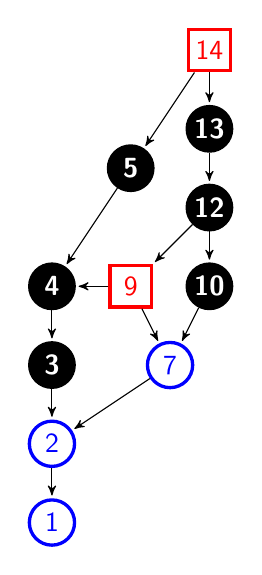
\begin{tikzpicture}[->,>=stealth',shorten >=1pt,auto,node distance=3cm,
  thick,main node/.style={circle,fill=blue!20,draw,font=\sffamily\Large\bfseries}]
  
  
  
  \node[arn_b] (a1) at (0,0) {1};
  \node[arn_b] (a2) at (0,1) {2};
  
  \node[arn_n] (a5) at (1,4.5) {5};
  \node[arn_n] (a13) at (2,5) {13};
  \node[arn_rs] (a14) at (2,6) {14};
  
  
  \node[arn_n] (a10) at (2,3) {10};
  \node[arn_b] (a7) at (1.5,2) {7};
  \node[arn_n] (a3) at (0,2) {3};
  
  \node[arn_rs] (a9) at (1,3) {9};
  \node[arn_n] (a12) at (2,4) {12};
  \node[arn_n] (a4) at (0,3) {4};
  
  %   Alice history
  \path[thin] (a14) edge (a5);
  \path[thin] (a5) edge (a4);
  \path[thin] (a4) edge (a3);
  \path[thin] (a3) edge (a2);
  \path[thin] (a2) edge (a1);
  \path[thin] (a9) edge (a4);
  \path[thin] (a7) edge (a2);
%   both history
  \path[thin] (a14) edge (a13);
  \path[thin] (a13) edge (a12);
  \path[thin] (a12) edge (a9);
  \path[thin] (a12) edge (a10);
  
  \path[thin] (a9) edge (a7);
  \path[thin] (a10) edge (a7);
  \end{tikzpicture}
  \caption{deal with bloomfilters}
\end{minipage}
 \begin{minipage}{0.3\textwidth}
 \centering
 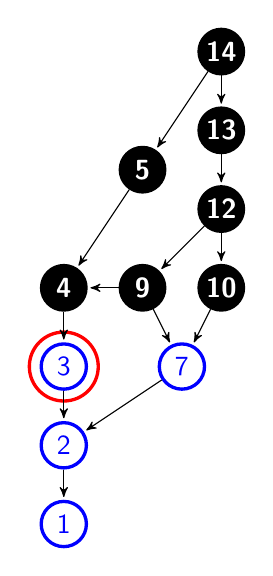
\begin{tikzpicture}[->,>=stealth',shorten >=1pt,auto,node distance=3cm,
  thick,main node/.style={circle,fill=blue!20,draw,font=\sffamily\Large\bfseries}]
  
  

  \node[arn_rb] (emph) at (0,2) {};
  \node[arn_b] (a1) at (0,0) {1};
  \node[arn_b] (a2) at (0,1) {2};
  
  \node[arn_n] (a5) at (1,4.5) {5};
  \node[arn_n] (a13) at (2,5) {13};
  \node[arn_n] (a14) at (2,6) {14};
  
  
  \node[arn_n] (a10) at (2,3) {10};
  \node[arn_b] (a7) at (1.5,2) {7};
  \node[arn_b] (a3) at (0,2) {3};
  
  \node[arn_n] (a9) at (1,3) {9};
  \node[arn_n] (a12) at (2,4) {12};
  \node[arn_n] (a4) at (0,3) {4};
%   \node[cloud, fill=gray!20, cloud puffs=16, cloud puff arc= 100,minimum width=2em, minimum height=2em, aspect=1] (cloud) at (5,2) {};

  %   Alice history
  \path[thin] (a14) edge (a5);
  \path[thin] (a5) edge (a4);
  \path[thin] (a4) edge (a3);
  \path[thin] (a3) edge (a2);
  \path[thin] (a2) edge (a1);
  \path[thin] (a9) edge (a4);
  \path[thin] (a7) edge (a2);
%   both history
  \path[thin] (a14) edge (a13);
  \path[thin] (a13) edge (a12);
  \path[thin] (a12) edge (a9);
  \path[thin] (a12) edge (a10);
  
  \path[thin] (a9) edge (a7);
  \path[thin] (a10) edge (a7);
  \end{tikzpicture}
  \caption{deal with border}
\end{minipage}
\end{figure}
\begin{figure}[H]
  \begin{minipage}{0.3\textwidth}
  \centering
 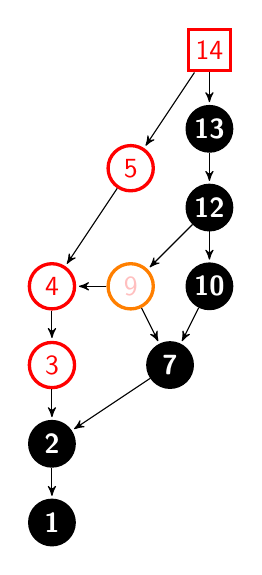
\begin{tikzpicture}[->,>=stealth',shorten >=1pt,auto,node distance=3cm,
  thick,main node/.style={circle,fill=blue!20,draw,font=\sffamily\Large\bfseries}]
  
  
  \node[arn_n] (a1) at (0,0) {1};
  \node[arn_n] (a2) at (0,1) {2};
  
  \node[arn_r] (a5) at (1,4.5) {5};
  \node[arn_n] (a13) at (2,5) {13};
  \node[arn_rs] (a14) at (2,6) {14};
  
  
  \node[arn_n] (a10) at (2,3) {10};
  \node[arn_n] (a7) at (1.5,2) {7};
  \node[arn_r] (a3) at (0,2) {3};
  
  \node[arn_t] (a9) at (1,3) {9};
  \node[arn_n] (a12) at (2,4) {12};
  \node[arn_r] (a4) at (0,3) {4};
%   \node[cloud, fill=gray!20, cloud puffs=16, cloud puff arc= 100,minimum width=2em, minimum height=2em, aspect=1] (cloud) at (5,2) {};

  %   Alice history
  \path[thin] (a14) edge (a5);
  \path[thin] (a5) edge (a4);
  \path[thin] (a4) edge (a3);
  \path[thin] (a3) edge (a2);
  \path[thin] (a2) edge (a1);
  \path[thin] (a9) edge (a4);
  \path[thin] (a7) edge (a2);
%   both history
  \path[thin] (a14) edge (a13);
  \path[thin] (a13) edge (a12);
  \path[thin] (a12) edge (a9);
  \path[thin] (a12) edge (a10);
  
  \path[thin] (a9) edge (a7);
  \path[thin] (a10) edge (a7);
  \end{tikzpicture}
  \caption{explore}
\end{minipage}
  \begin{minipage}{0.3\textwidth}
  \centering
 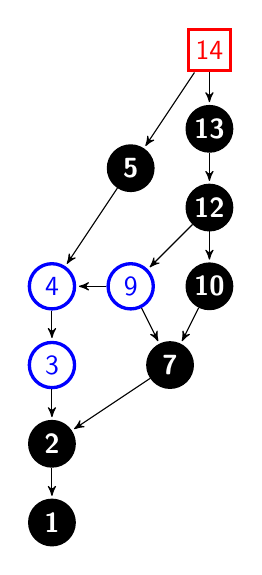
\begin{tikzpicture}[->,>=stealth',shorten >=1pt,auto,node distance=3cm,
  thick,main node/.style={circle,fill=blue!20,draw,font=\sffamily\Large\bfseries}]
  
  
  \node[arn_n] (a1) at (0,0) {1};
  \node[arn_n] (a2) at (0,1) {2};
  
  \node[arn_n] (a5) at (1,4.5) {5};
  \node[arn_n] (a13) at (2,5) {13};
  \node[arn_rs] (a14) at (2,6) {14};
  
  
  \node[arn_n] (a10) at (2,3) {10};
  \node[arn_n] (a7) at (1.5,2) {7};
  \node[arn_b] (a3) at (0,2) {3};
  
  \node[arn_b] (a9) at (1,3) {9};
  \node[arn_n] (a12) at (2,4) {12};
  \node[arn_b] (a4) at (0,3) {4};
%   \node[cloud, fill=gray!20, cloud puffs=16, cloud puff arc= 100,minimum width=2em, minimum height=2em, aspect=1] (cloud) at (5,2) {};

  %   Alice history
  \path[thin] (a14) edge (a5);
  \path[thin] (a5) edge (a4);
  \path[thin] (a4) edge (a3);
  \path[thin] (a3) edge (a2);
  \path[thin] (a2) edge (a1);
  \path[thin] (a9) edge (a4);
  \path[thin] (a7) edge (a2);
%   both history
  \path[thin] (a14) edge (a13);
  \path[thin] (a13) edge (a12);
  \path[thin] (a12) edge (a9);
  \path[thin] (a12) edge (a10);
  
  \path[thin] (a9) edge (a7);
  \path[thin] (a10) edge (a7);
  \end{tikzpicture}
  \caption{deal with bloomfilters}
\end{minipage}
\begin{minipage}{0.3\textwidth}
  \centering
 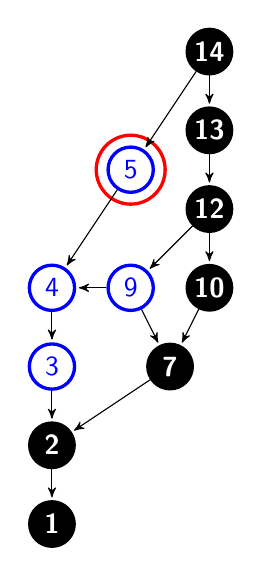
\begin{tikzpicture}[->,>=stealth',shorten >=1pt,auto,node distance=3cm,
  thick,main node/.style={circle,fill=blue!20,draw,font=\sffamily\Large\bfseries}]
  
  \node[arn_rb] (emph) at (1,4.5) {};
  \node[arn_n] (a1) at (0,0) {1};
  \node[arn_n] (a2) at (0,1) {2};
  
  \node[arn_b] (a5) at (1,4.5) {5};
  \node[arn_n] (a13) at (2,5) {13};
  \node[arn_n] (a14) at (2,6) {14};
  
  
  \node[arn_n] (a10) at (2,3) {10};
  \node[arn_n] (a7) at (1.5,2) {7};
  \node[arn_b] (a3) at (0,2) {3};
  
  \node[arn_b] (a9) at (1,3) {9};
  \node[arn_n] (a12) at (2,4) {12};
  \node[arn_b] (a4) at (0,3) {4};
%   \node[cloud, fill=gray!20, cloud puffs=16, cloud puff arc= 100,minimum width=2em, minimum height=2em, aspect=1] (cloud) at (5,2) {};

  %   Alice history
  \path[thin] (a14) edge (a5);
  \path[thin] (a5) edge (a4);
  \path[thin] (a4) edge (a3);
  \path[thin] (a3) edge (a2);
  \path[thin] (a2) edge (a1);
  \path[thin] (a9) edge (a4);
  \path[thin] (a7) edge (a2);
%   both history
  \path[thin] (a14) edge (a13);
  \path[thin] (a13) edge (a12);
  \path[thin] (a12) edge (a9);
  \path[thin] (a12) edge (a10);
  
  \path[thin] (a9) edge (a7);
  \path[thin] (a10) edge (a7);
  \end{tikzpicture}
  \caption{deal with borders}
\end{minipage}
\end{figure}
\begin{figure}[H]
 
\begin{minipage}{0.3\textwidth}
  \centering
 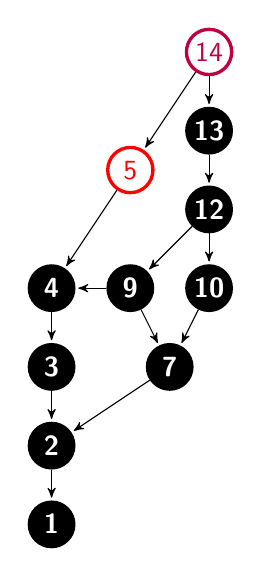
\begin{tikzpicture}[->,>=stealth',shorten >=1pt,auto,node distance=3cm,
  thick,main node/.style={circle,fill=blue!20,draw,font=\sffamily\Large\bfseries}]
  
  
  \node[arn_n] (a1) at (0,0) {1};
  \node[arn_n] (a2) at (0,1) {2};
  
  \node[arn_r] (a5) at (1,4.5) {5};
  \node[arn_n] (a13) at (2,5) {13};
  \node[arn_pu] (a14) at (2,6) {14};
  
  
  \node[arn_n] (a10) at (2,3) {10};
  \node[arn_n] (a7) at (1.5,2) {7};
  \node[arn_n] (a3) at (0,2) {3};
  
  \node[arn_n] (a9) at (1,3) {9};
  \node[arn_n] (a12) at (2,4) {12};
  \node[arn_n] (a4) at (0,3) {4};
%   \node[cloud, fill=gray!20, cloud puffs=16, cloud puff arc= 100,minimum width=2em, minimum height=2em, aspect=1] (cloud) at (5,2) {};

  %   Alice history
  \path[thin] (a14) edge (a5);
  \path[thin] (a5) edge (a4);
  \path[thin] (a4) edge (a3);
  \path[thin] (a3) edge (a2);
  \path[thin] (a2) edge (a1);
  \path[thin] (a9) edge (a4);
  \path[thin] (a7) edge (a2);
%   both history
  \path[thin] (a14) edge (a13);
  \path[thin] (a13) edge (a12);
  \path[thin] (a12) edge (a9);
  \path[thin] (a12) edge (a10);
  
  \path[thin] (a9) edge (a7);
  \path[thin] (a10) edge (a7);
  \end{tikzpicture}
  \caption{explore}
\end{minipage}
\begin{minipage}{0.3\textwidth}
  \centering
 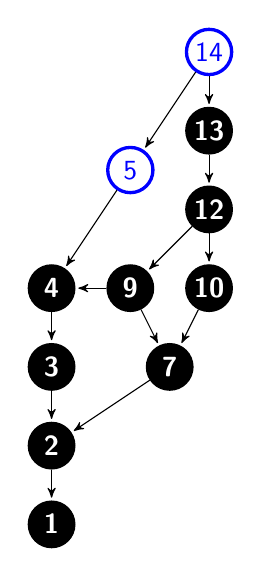
\begin{tikzpicture}[->,>=stealth',shorten >=1pt,auto,node distance=3cm,
  thick,main node/.style={circle,fill=blue!20,draw,font=\sffamily\Large\bfseries}]
  
  
  \node[arn_n] (a1) at (0,0) {1};
  \node[arn_n] (a2) at (0,1) {2};
  
  \node[arn_b] (a5) at (1,4.5) {5};
  \node[arn_n] (a13) at (2,5) {13};
  \node[arn_b] (a14) at (2,6) {14};
  
  
  \node[arn_n] (a10) at (2,3) {10};
  \node[arn_n] (a7) at (1.5,2) {7};
  \node[arn_n] (a3) at (0,2) {3};
  
  \node[arn_n] (a9) at (1,3) {9};
  \node[arn_n] (a12) at (2,4) {12};
  \node[arn_n] (a4) at (0,3) {4};
%   \node[cloud, fill=gray!20, cloud puffs=16, cloud puff arc= 100,minimum width=2em, minimum height=2em, aspect=1] (cloud) at (5,2) {};

  %   Alice history
  \path[thin] (a14) edge (a5);
  \path[thin] (a5) edge (a4);
  \path[thin] (a4) edge (a3);
  \path[thin] (a3) edge (a2);
  \path[thin] (a2) edge (a1);
  \path[thin] (a9) edge (a4);
  \path[thin] (a7) edge (a2);
%   both history
  \path[thin] (a14) edge (a13);
  \path[thin] (a13) edge (a12);
  \path[thin] (a12) edge (a9);
  \path[thin] (a12) edge (a10);
  
  \path[thin] (a9) edge (a7);
  \path[thin] (a10) edge (a7);
  \end{tikzpicture}
  \caption{deal with bloomfilters}
\end{minipage}
\begin{minipage}{0.3\textwidth}
  \centering
 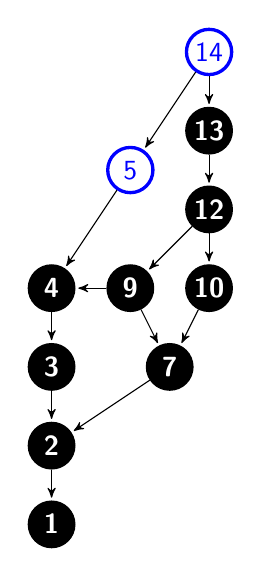
\begin{tikzpicture}[->,>=stealth',shorten >=1pt,auto,node distance=3cm,
  thick,main node/.style={circle,fill=blue!20,draw,font=\sffamily\Large\bfseries}]
  
  
  \node[arn_n] (a1) at (0,0) {1};
  \node[arn_n] (a2) at (0,1) {2};
  
  \node[arn_b] (a5) at (1,4.5) {5};
  \node[arn_n] (a13) at (2,5) {13};
  \node[arn_b] (a14) at (2,6) {14};
  
  
  \node[arn_n] (a10) at (2,3) {10};
  \node[arn_n] (a7) at (1.5,2) {7};
  \node[arn_n] (a3) at (0,2) {3};
  
  \node[arn_n] (a9) at (1,3) {9};
  \node[arn_n] (a12) at (2,4) {12};
  \node[arn_n] (a4) at (0,3) {4};
%   \node[cloud, fill=gray!20, cloud puffs=16, cloud puff arc= 100,minimum width=2em, minimum height=2em, aspect=1] (cloud) at (5,2) {};

  %   Alice history
  \path[thin] (a14) edge (a5);
  \path[thin] (a5) edge (a4);
  \path[thin] (a4) edge (a3);
  \path[thin] (a3) edge (a2);
  \path[thin] (a2) edge (a1);
  \path[thin] (a9) edge (a4);
  \path[thin] (a7) edge (a2);
%   both history
  \path[thin] (a14) edge (a13);
  \path[thin] (a13) edge (a12);
  \path[thin] (a12) edge (a9);
  \path[thin] (a12) edge (a10);
  
  \path[thin] (a9) edge (a7);
  \path[thin] (a10) edge (a7);
  \end{tikzpicture}
  \caption{deal with borders}
\end{minipage}
\end{figure}

\end{document}

